\documentclass[portuguese]{textolivre}

% metadata
\journalname{Texto Livre}
\thevolume{18}
%\thenumber{1} % old template
\theyear{2025}
\receiveddate{\DTMdisplaydate{2024}{11}{8}{-1}}
\accepteddate{\DTMdisplaydate{2025}{1}{30}{-1}}
\publisheddate{\DTMdisplaydate{2025}{4}{9}{-1}}
\corrauthor{Gabriel Esteves}
\articledoi{10.1590/1983-3652.2025.55787}
%\articleid{NNNN} % if the article ID is not the last 5 numbers of its DOI, provide it using \articleid{} commmand 
% list of available sesscions in the journal: articles, dossier, reports, essays, reviews, interviews, editorial
\articlesessionname{articles}
\runningauthor{Esteves, Scarabelot e Sousa}
%\editorname{Leonardo Araújo} % old template
\sectioneditorname{Daniervelin Pereira}
\layouteditorname{Leonardo Araújo}

\title{Verso romântico? Revisitando o decassílabo sáfico com ferramentas digitais}
\othertitle{Romantic verse? Revisiting the sapphic decasyllable with digital tools}

\author[1]{Gabriel Esteves~\orcid{0000-0003-4719-6672}\thanks{Email: \href{mailto:gabrielesteues@gmail.com}{gabrielesteues@gmail.com}}}
\author[1]{Leandro Scarabelot~\orcid{0000-0003-4151-4924}\thanks{Email: \href{mailto:leandro-scarabelot@hotmail.com}{leandro-scarabelot@hotmail.com}}}
\author[1]{Ana Paula Nunes de Sousa~\orcid{0000-0002-9971-311X}\thanks{Email: \href{mailto:anapaulacxs1234@gmail.com}{anapaulacxs1234@gmail.com}}}
\affil[1]{Universidade Federal de Santa Catarina, Florianópolis, SC, Brasil.}

\addbibresource{article.bib}

\begin{document}
\maketitle
\begin{polyabstract}
\begin{abstract}
No campo dos estudos literários, o método quantiqualitativo, conhecido como estilometria literária e estatística textual, vem ganhando destaque. Esse tipo de pesquisa se caracteriza pelo uso de ferramentas computacionais no contexto da cultura digital, que realizam análises rápidas e precisas de elementos estilísticos para identificar autores, poetas e escolas literárias. Este trabalho revisa a hipótese de que o decassílabo sáfico seria uma marca distintiva da poesia romântica brasileira. Usamos a ferramenta digital Aoidos para a escansão automática dos versos, obtendo dados quantitativos sobre o tamanho e ritmo dos versos. Comparando o uso de tipos de decassílabo (sáfico, heroico e andrógino) entre quatro grupos de poetas (neoclássicos, românticos, geração de 1870 e parnasianos), verificamos que, apesar de um aumento de quase 75\% no uso desse verso do século XVIII para o XIX, ele não é traço exclusivo dos poetas românticos, o que nos permite concluir que a percepção do uso exacerbado de sáficos decorre de algumas obras específicas, não de um fenômeno generalizado. Essa análise permite questionar interpretações tradicionais de autores como Antonio Candido e Péricles Eugênio da Silva Ramos, que veem no sáfico uma característica central da poesia romântica. Concluímos que a hipótese de predomínio do verso sáfico no romantismo carece de respaldo empírico, já que ele atravessa diferentes movimentos literários de maneira relativamente estável ao longo do século XIX.

\keywords{Estudo quantiqualitativo \sep Estatística textual \sep Ferramentas digitais \sep Verso romântico \sep Decassílabo sáfico}
\end{abstract}

\begin{english}
\begin{abstract}
In the field of literary studies, the quanti-qualitative method, known as literary stylometry and textual statistics, has gained prominence. This type of research is characterized by the use of computational tools in the context of digital culture, performing rapid and precise analyses of stylistic elements to identify authors, poets, and literary schools. This study revisits the hypothesis that the Sapphic decasyllable is a distinctive mark of Brazilian Romantic poetry. We use the digital tool Aoidos for automatic verse scansion, obtaining quantitative data on verse length and rhythm. By comparing the use of different types of decasyllable (Sapphic, heroic, and androgynous) across four groups of poets (Neoclassical, Romantic, Generation of 1870, and Parnassian), we observed that, despite an increase of nearly 75\% in the use of this verse type from the 18th to the 19th century, it is not an exclusive trait of Romantic poets. This finding allows us to conclude that the perception of excessive Sapphic usage stems from certain specific works rather than a widespread phenomenon. This analysis raises questions about traditional interpretations by critics such as Antonio Candido and Péricles Eugênio da Silva Ramos, who view the Sapphic as a central feature of Romantic poetry. We conclude that the hypothesis of Sapphic verse predominance in Romanticism lacks empirical support, as it traverses various literary movements with relative stability throughout the 19th century.

\keywords{Quanti-qualitative study \sep Textual statistics \sep Digital tools \sep Romantic verse \sep Sapphic Decasyllable}
\end{abstract}
\end{english}
\end{polyabstract}

\section{Introdução}
Quando se fala em versificação romântica no Brasil, há uma conhecida hipótese que vem sempre à tona, e que tem passado incontestada de uma a outra geração de historiadores literários: a suposta predileção dos poetas identificados com o romantismo pelo verso decassílabo acentuado nas 4ª e 8ª sílabas, ou seja, suposta predileção pelo verso sáfico — musical, envolvente, pé de valsa, avesso à \textit{bienséance} neoclássica. Não são poucos nem desconhecidos os defensores dessa leitura. Ratificam-na importantes críticos da poesia nacional como Antonio Candido, Péricles Eugênio da Silva Ramos e José Guilherme Merquior. Trata-se, portanto, de uma hipótese consagrada, de um lugar comum da nossa historiografia literária.

Péricles Eugênio da Silva Ramos, por exemplo, no livro \textit{O verso romântico e outros ensaios} \cite[p.~9]{ramos1959verso}, afirma categoricamente que os poetas românticos fizeram “emprego insistente” do esquema sáfico, que “poesias assim são banais entre os românticos brasileiros” \cite[p.~26]{ramos1959verso}, e repete o argumento em outras duas ocasiões: no capítulo “A renovação parnasiana na poesia”, escrito para a coleção \textit{A literatura no Brasil} — “o verso decassílabo, muitas vezes monótono entre os românticos, que o usavam insistentemente com o esquema sáfico” \cite[p.~128]{ramos1969renovacao} —; e em \textit{Do barroco ao modernismo} \cite{ramos1968barroco}, onde argumenta que os poetas românticos, alastrando o verso sáfico “por poesias inteiras”, consolidaram uma tradição versificatória à parte, sem continuidade imediata nos movimentos posteriores \cite[p.~74]{ramos1968barroco}, que eclipsariam o “uso uniforme do decassílabo sáfico” \cite[p.~162]{ramos1989introducao}.

Antonio Candido, por sua vez, em diversos volumes, eleva a interpretação de Silva Ramos a um novo patamar especulativo, chegando a propor uma interpretação estético-sociológica para o fenômeno: “tiveram os românticos predileção marcada e significativa pelo [decassílabo] de acentuação nas 4ª, 8ª e 10ª, o verso ‘sáfico’”, cuja musicalidade exploraram até o fastio, até a monotonia, incorporando-o “ao que havia de mais característico na sua estética” e banalizando-o até o nível da “valsinha de salão” \cite[p.~36]{candido2000formacao}, da “melopeia automática e sem fibra” \cite[p.~221]{candido2000formacao}. Engajados na luta pela valorização da sensibilidade contra a tirania da razão, queriam ferir em cheio as “reservas dos tratadistas e do gosto anterior, [...] em consonância à mudança de concepções que acompanhou as grandes mudanças sociais do século XVIII na sua passagem para o XIX” \cite[p.~56]{candido1996estudo}. Essa “invasão de melodia no verso”, como chama Antonio Candido à suposta mudança de paradigma efetuada pelos poetas românticos, está melhor descrita (e datada: a partir de Casimiro de Abreu) no pequeno volume \textit{O romantismo no Brasil} \cite[p.~64-65]{candido2002romantismo}:

\begin{quote}
    Assim, o decassílabo sáfico [...], antes usado com parcimônia, assume, a partir de Casimiro de Abreu, uma espécie de indiscreta preeminência, por ocorrer, ao contrário do que recomendavam os tratadistas de poética, em todos os versos do poema, de maneira a criar melopeias que envolvem a sensibilidade como encantamento, superpondo-se ao próprio sentido. O seu airoso movimento de valsa transforma o texto em dança e parece querer suprir a insuficiência da palavra com auxílio de sua música infusa. A isso se junta o gosto pela rima interna, que aumenta a sonorização e envolve o leitor, ou auditor, numa espécie de entorpecimento que anestesia a razão. Essa é, aliás, uma tendência comum a toda poesia de língua portuguesa daquele tempo, e foi com os poetas de Além-Mar que os brasileiros aprenderam a segui-la. [...] O sáfico invariável, cujo emprego culmina nos anos 60 e 70, produz um ritmo mais melodioso e serve para muitos matizes do sentimento lírico. É preciso lembrar que nos anos 60 foi intensa a aliança entre música e poesia, não apenas por meio dos recitativos acompanhados ao piano por um apoio sonoro, mas pelo hábito cada vez mais difundido de musicar os poemas…
\end{quote}

José Guilherme Merquior reitera o argumento de seus predecessores, em especial o de Antonio Candido, frisando que os versos preferidos pelos românticos, entre os quais se destaca o decassílabo sáfico, dissolvidos em ritmos cantantes e automáticos apropriados aos saraus oitocentistas, tendiam muitas vezes “a converter-se em pura \textit{melopeia}” \cite[p.~74]{merquior1979anchieta}.

Vê-se, assim, que a historiografia literária brasileira (e portuguesa!\footnote{Amorim de Carvalho, por exemplo, autor de uma \textit{Teoria geral da versificação} \cite{carvalho1987teoria}, não hesita em escrever que o decassílabo sáfico, de uso moderado até o século XIX, sempre alternado com o decassílabo heroico, começa a ser empregado “com inteira autonomia” durante o período romântico pelo seu “prestígio musical” característico: “era um ritmo cantante que se casava bem com a expressão lírica e intensiva da alma romântica” \cite[p.~286]{carvalho1987teoria}.}) tem reiteradamente apresentado o decassílabo sáfico como um verso característico da poética romântica, e prescindindo muitas vezes de demonstração, como se tratássemos de um fato. Pesquisas recentes, contudo, desenvolvidas com o auxílio de ferramentas de processamento textual, têm servido à contestação dessa hipótese. \textcite{sousa2023teofilo}, por exemplo, em sua dissertação de mestrado, \textit{Teófilo Dias e a poética parnasiana: estudo estilométrico} \cite[p.~100]{sousa2023teofilo}, sugere que alguns poetas parnasianos como Alberto de Oliveira e Olavo Bilac manifestam uma sutil preferência pelo decassílabo sáfico, enquanto o romântico Álvares de Azevedo parece se inclinar sensivelmente ao uso do decassílabo heroico. Já \textcite{scarabelot2024poetas}, em sua tese de doutorado, \textit{Os poetas realistas da geração de 1870: uma geração poeticamente perdida?}, demonstra que o percentual de decassílabos sáficos é praticamente o mesmo entre poetas românticos, realistas e parnasianos, enquanto que o emprego proporcional de decassílabos heroicos, supostamente menor entre os românticos, é equiparável ao dos poetas da geração de 70 e muito superior ao dos parnasianos.

À luz dessas novas evidências, passamos a suspeitar que a hipótese do sáfico romântico apresentasse lacunas e estivesse fundamentada em impressões de leitura subjetivas. Decidimos, assim, pô-la à prova uma vez mais e verificar se as ideias de Candido, Silva Ramos e Merchior são respaldadas por dados quantitativos. Com a ajuda de uma ferramenta de processamento automático de textos desenvolvida por Adiel Mittmann e pelo Núcleo de Pesquisas em Informática, Literatura e Linguística (NuPILL) da Universidade Federal de Santa Catarina, o Aoidos (\url{https://aoidos.ufsc.br/}), investigamos se o uso do decassílabo sáfico pode ou não ser considerado um traço distintivo da versificação romântica brasileira como um todo e descobrimos que, embora haja um crescimento significativo na utilização desse tipo de verso na transição do século XVIII para o XIX, sua presença se mantém proporcionalmente estável ao longo do século XIX, atravessando o romantismo, a geração de 70 e o parnasianismo sem grandes alterações, conforme se verá a seguir.

\section{Corpus e método de análise}\label{sec-normas}
Nos últimos anos, o emprego de ferramentas digitais tem produzido importantes contribuições para pesquisas na área dos estudos literários e, em especial, nas áreas da historiografia literária e da estilometria\footnote{O fenômeno é notável, por exemplo, em pesquisas ligadas à poesia. Nessa área, diversos artigos, dissertações e teses têm sido produzidos a partir do uso de ferramentas digitais nos últimos dez anos. Dentre os artigos escritos por autores brasileiros, podemos citar: “Análise comparativa entre as escansões manual e automática dos versos de Gregório de Matos” \cite{mittmann2017analise}; “The Rhythm of Epic Verse in Portuguese from the 16th to the 21st century” \cite{mittmann2018rhythm}; “Peeking inside the rhythmic possibilities of the portuguese decassílabo” \cite{mittmann2021peeking}; “What rhythmic signature says about poetic corpora” \cite{mittmann2019rhythmic}. Dentre as dissertações e teses de autores brasileiros, podemos citar: "Ritmos sem qualidades: leituras em versus de uma vertente da poesia portuguesa contemporânea" \cite{osorio2019ritmos}; "Teófilo Dias e a poética parnasiana: estudo estilométrico" \cite{sousa2023teofilo}; e "Os poetas realistas da geração de 1870: uma geração poeticamente perdida?" \cite{scarabelot2024poetas}.}. Apesar dos resultados positivos, o campo ainda enfrenta uma dificuldade que a pesquisa convencional, o \textit{tête-à-tête} com o livro físico, não possui: a necessidade de que as obras estejam em determinado formato digital. Quando se estuda algo tão específico como a poesia brasileira dos séculos XVIII e XIX, ou, mais precisamente, a produção poética entre os períodos neoclássico e parnasiano, a dificuldade parece aumentar. Para melhor compreender o problema, vejamos alguns dados.

Dentre os mais de 85 mil documentos cadastrados na Biblioteca Digital de Literatura de Países Lusófonos (BLPL), apenas 11.352 estão em formato digital. Quando refinamos a pesquisa, estabelecendo como critério de busca o “país de nascimento” (Brasil), o “gênero literário” (poema) e o “ano de publicação” (1768-1921), encontramos um total de 3.654 obras cadastradas, dentre as quais apenas 1.061 estão em formato digital. Os números diminuem ainda mais se nos atentamos ao fato de que a BLPL não distingue entre poemas avulsos publicados em periódicos e livros propriamente ditos, o que faz com que a quantidade destes últimos seja ainda menor. Assim sendo, embora nós mesmos tenhamos digitalizado algumas obras disponíveis fisicamente na Fundação Biblioteca Nacional, nossa pesquisa se baseou quase estritamente em obras que já estavam disponíveis em formato digital (PDF ou HTML).

Tendo as obras em formato digital, utilizamos um mecanismo de reconhecimento ótico de caracteres (OCR) para convertê-las em textos editáveis e atualizá-las ortograficamente, sempre em cotejo com os originais. Logo após, transpusemo-las para o formato XML (\textit{Extensible Markup Language}), linguagem utilizada para o processamento e análise dos dados pelo Aoidos, ferramenta digital online e gratuita que faz escansão automática de versos, gerando dados estatísticos em relação aos metros e ritmos utilizados, bem como aos processos de acomodação silábica (metaplasmos) utilizados pelos(as) poetas.

Considerando nossa hipótese de que o decassílabo sáfico não se configura como um traço distintivo dos poetas românticos em relação a outras escolas literárias, selecionamos um corpus composto por obras de autores divididos em quatro grupos distintos, conforme a classificação historiográfica dos movimentos literários\footnote{Para a distribuição dos poetas e de suas respectivas obras em determinados movimentos literários, baseamo-nos nas indicações de nossos principais historiadores literários, como Sílvio Romero, José Veríssimo, Péricles Eugênio da Silva Ramos, Antonio Candido, Alfredo Bosi e Luciana Stegagno-Picchio. Vale salientar que, por considerarmos mais importante o \textit{conteúdo} da obra, alguns autores estão inseridos em mais de um movimento literário.}: neoclássicos, românticos, geração de 1870 e parnasianos.

As obras que compõem o grupo dos poetas neoclássicos são: \textit{Caramuru} (1781), de Santa Rita Durão; \textit{Obras} (1768) e \textit{Vila Rica} (1773), de Cláudio Manuel da Costa; \textit{Marília de Dirceu} (1792) e \textit{Cartas Chilenas} (1845)\footnote{A fim de esclarecimento, não objetivamos entrar na discussão acerca da autoria das \textit{Cartas Chilenas}. Aqui, vale mencionar o trabalho de \textcite{brandao2006atribuicao}, “Atribuição de autoria: um problema antigo, novas ferramentas”. Nele, o pesquisador realizou, por meio da ferramenta digital LEXICO3, um estudo estatístico-computacional cujo objetivo consistiu em verificar a verdadeira autoria das \textit{Cartas Chilenas}, que é atribuída a Tomás Antônio Gonzaga.}, de Tomás Antônio Gonzaga; \textit{O Uraguai} (1769), de Basílio da Gama; e \textit{O Desertor} (1774), de Silva Alvarenga.

Com relação às obras que compõem o grupo dos poetas românticos, elas são: \textit{Suspiros poéticos e saudades} (1836), de Gonçalves de Magalhães; a “Nênia à morte do meu bom amigo o Dr. Francisco Bernardino Ribeiro” (1841), de Firmino Rodrigues da Silva; \textit{Primeiros Cantos} (1846), \textit{Últimos Cantos} (1851) e \textit{Os Timbiras} (1861), de Gonçalves Dias; \textit{Lira dos vinte anos} (1853), de Álvares de Azevedo; \textit{As primaveras} (1859), de Casimiro de Abreu; Noturnas (1861) e \textit{Anchieta} (1875), de Fagundes Varela; \textit{Lírios e Rosas} (1863), de José Eliziário; \textit{Corimbos} (1869), de Luís Guimarães Júnior; \textit{Espumas flutuantes} (1870), \textit{A Cachoeira de Paulo Afonso} (1876 [1871]) e \textit{Os escravos} (1884 [1871]), de Castro Alves; \textit{Versos} (1870), de Celso da Cunha Magalhães; \textit{Peregrinas} (1870), de Vitoriano Palhares; \textit{Rosas loucas} (1871), de Carlos Ferreira; \textit{Poesias} (1871), de Jaime Augusto de Castro; \textit{Fábio} (1871), de Joaquim Serra; \textit{Sertanejas} (1873), de Joaquim Eleodoro; \textit{Quadros} (1873), de Joaquim Serra; \textit{Gritos da Carne} (1874), de José Leão; \textit{Peregrinas} (1874), de Otaviano Hudson; \textit{Estrelas errantes} (1876), de Quirino dos Santos; \textit{Miosótis} (1877), de Teixeira de Melo; e \textit{Dias e noites} (1881), de Tobias Barreto.

Quanto às obras que compõem o grupo dos poetas ligados à geração de 70, temos: \textit{Flores do campo} (1874), de Ezequiel Freire; \textit{Prelúdios} (1876) e \textit{Devaneios} (1876), de Afonso Celso Júnior; \textit{Canções românticas} (1878), de Alberto de Oliveira, bem como os poemas “O caixeiro” e “Rosa” (1878), publicados sob o pseudônimo Atta-Troll4; \textit{Cantos do fim do século} (1878), de Sílvio Romero; \textit{Hespérides} (1879), de Carvalho Júnior; \textit{Auroras do sul} (1879), de Damasceno Vieira; \textit{Cantos e Lutas} (1879), de Valentim Magalhães; \textit{Novos ideais} (1880), de Múcio Teixeira; \textit{Fanfarras} (1882), de Teófilo Dias; \textit{Sinfonias} (1883), de Raimundo Correia; Opalas (1884), de Fontoura Xavier; \textit{Estilhaços} (1885), de Isidoro Martins Júnior; e \textit{Vergastas} (1889), de Lúcio de Mendonça.

Por fim, as obras que compõem o grupo dos poetas parnasianos são: \textit{Cromos} (1896 [1881]), de B. Lopes; \textit{Meridionais} (1900 [1884]), \textit{Sonetos e poemas} (1885) e \textit{Poesias: 2ª série} (1892), de Alberto de Oliveira; \textit{Sonetos e rimas} (1886), de Luís Guimarães Júnior; \textit{Versos e versões} (1887) e \textit{Poesias} (1922 [1902]), de Raimundo Correia; \textit{Versos de um simples} (1891), de Guimarães Passos; \textit{Mármores} (1895) e \textit{Esfinges} (1921), de Francisca Júlia; \textit{Poesias} (1902) e \textit{Tarde} (1919), de Olavo Bilac; \textit{Vibrações} (1905), de Júlia Cortines; e \textit{Ementário} (1908), de Gustavo Teixeira.


\section{Discussão dos resultados}\label{sec-conduta}
Conforme mencionado, o Aoidos faz o levantamento automático dos esquemas rítmicos dispostos em um determinado corpus. Entretanto, ele não nomeia esses esquemas rítmicos segundo a nomenclatura tradicional da versificação de língua portuguesa. A tradução desses dados quantitativos para a terminologia empregada nos manuais poéticos (ou quaisquer outras terminologias) é uma tarefa posterior e subjetiva, realizada de acordo com os critérios escolhidos por cada pesquisador, o que pode levar a desentendimentos definicionais. Especifiquemos, desse modo, a fim de evitar controvérsias, quais esquemas rítmicos consideramos sáficos e quais consideramos heroicos.

Consideramos um verso como sáfico se seus acentos principais recaem nas sílabas 4ª e 10ª, mas não na 6ª (acento do verso heroico). Quanto à acentuação na 8ª sílaba, marca tradicional do decassílabo sáfico na obra de inúmeros tratadistas, julgamo-la dispensável. Isso porque, conforme afirma \textcite[p.~58]{proenca1955ritmo}, a característica fundamental do sáfico não é a acentuação na 8ª sílaba, mas a acentuação obrigatória na 4ª, sendo aquela apenas uma pausa provável e flutuante. Será sáfico, portanto, o verso cujo esquema rítmico contemple alguma dessas variações: 2-4-8-10, 1-4-8-10, 4-8-10, 2-4-10, 1-4-10 e 4-10.

Do mesmo modo, um verso é heroico quando seus acentos principais recaem nas sílabas 6ª e 10ª, mas não na 4ª (acento do verso sáfico). Se um verso for acentuado ao mesmo tempo nas sílabas 4ª e 6ª, não será considerado heroico, nem sáfico, mas \textit{andrógino}, já que essa dupla acentuação produz uma ambiguidade rítmica que permite ao leitor enfatizar um ou outro acento, a depender dos versos anteriores e posteriores, conforme postula \textcite{carvalho1987teoria} ao tratar da “lei da subordinação rítmica”, da “tonicidade posicional” e do “ritmo mais forte”. Assim sendo, será heroico o verso cujo esquema rítmico contemple alguma dessas variações: 3-6-10, 3-6-8-10, 2-6-8-10, 2-6-10, 1-3-6-10, 1-3-6-8-10, 1-6-8-10, 1-6-10, 6-8-10, 6-10. 

Falamos há pouco em verso andrógino como um verso ambíguo, ao mesmo tempo acentuado nas 4ª e 6ª sílabas. Esclareçamos. Trata-se de um tipo meramente virtual de verso, pois “o eventual verso andrógino pode ser ‘sexualizado’ a critério de quem o está escandindo, que decidirá pela cesura masculina ou feminina” \cite[p.~72]{mattoso2010sexo}. Ou seja, limitado a uma existência apenas hipotética, cabe ao leitor decidir se realiza o decassílabo andrógino, no ato da leitura, como heroico ou sáfico. Neste estudo, o andrógino foi incluído como tipo possível de decassílabo a fim de evitar ambiguidades e de tornar objetiva a distinção entre versos incontestavelmente sáficos e heroicos, uma vez que a realização de versos simultaneamente acentuados nas sílabas 4ª e 6ª poderia, dependendo de cada leitura subjetiva, alterar os resultados em favor de um ou de outro lado. Assim, será considerado andrógino todo verso que apresente um dos seguintes esquemas rítmicos: 2-4-6-10, 1-4-6-10, 2-4-6-8-10, 1-4-6-8-10, 4-6-10, 4-6-8-10.

Dito isso, vejamos, na \Cref{tbl1}, quais foram os resultados gerados pelo Aoidos quanto à disposição dos decassílabos heroicos, sáficos e andróginos nas obras dos poetas neoclássicos:

\begin{table}[htbp]
\centering
\begin{threeparttable}
\caption{Disposição dos decassílabos heroicos, sáficos e andróginos nos neoclássicos.}
\label{tbl1}
\begin{tabular}{llll}
\toprule
Obras & \multicolumn{3}{l}{Decassílabos nos neoclássicos} \\
& Heroicos & Sáficos & Andróginos \\
\midrule
\textit{Caramuru} & 48,5\% & 14,2\% & 37,2\% \\ 
\textit{Cartas Chilenas} & 64,7\% & 5,2\% & 30,1\% \\
\textit{Vila Rica} & 48,2\% & 14,9\% & 36,7\% \\
\textit{Marília de Dirceu} & 45,6\% & 9,2\% & 44,8\% \\
\textit{O Desertor} & 48,0\% & 12,2\% & 39,5\% \\
\textit{O Uraguai} & 46,0\% & 20,9\% & 32,8\% \\
\textit{Obras de C.M. da C.} & 49,1\% & 7,9\% & 42,9\% \\
\bottomrule
\end{tabular}
\source{Aoidos.}
\end{threeparttable}
\end{table}

Com relação ao emprego geral dos decassílabos heroicos, notamos que ele é sempre superior ao dos sáficos e andróginos, mesmo em casos limítrofes como o da \textit{Marília de Dirceu}, em que o uso do heroico supera o do andrógino em menos de  1\%. Trata-se, portanto, do verso mais utilizado pelos poetas neoclássicos, totalizando 48,2\% das ocorrências quando somamos os resultados da \Cref{tbl1} (\Cref{fig1}).

\begin{figure}[!h]
    \centering
    \begin{minipage}{0.75\linewidth}
    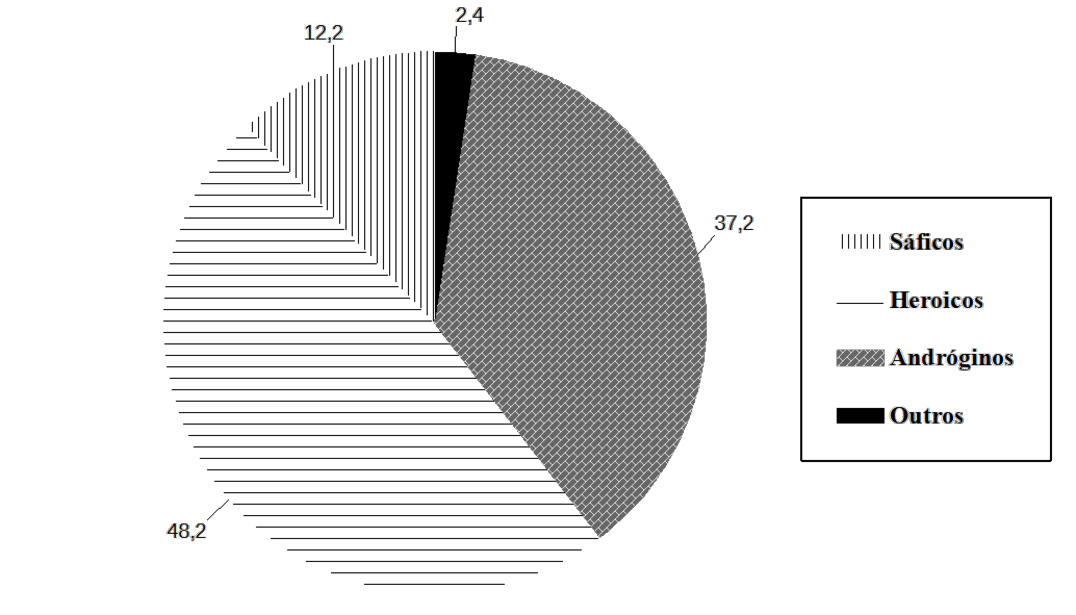
\includegraphics[width=\linewidth]{fig-001.pdf}
    \caption{Soma total dos tipos de decassílabo utilizados pelos neoclássicos.}
    \label{fig1}
    \source{Aoidos}
    \end{minipage}
\end{figure}

Quanto ao emprego do verso sáfico, observamos que ele representa apenas uma pequena parcela das ocorrências totais (12,2\%), mas apresenta variações individuais consideráveis se comparamos as ocorrências entre os poetas que compõem o grupo. Tomás Antônio Gonzaga, por exemplo, nunca ultrapassa os 10\% no emprego dos sáficos (5,2\% em \textit{Cartas Chilenas}; 9,2\% em \textit{Marília de Dirceu}), o que não ocorre quando olhamos para a obra de Cláudio Manuel da Costa, na qual a diferença entre os 7,9\% das Obras e os 14,9\% de Vila Rica (quase o dobro) reflete uma tendência maior, no segundo título, para a desambiguização dos versos andróginos. É o mesmo fenômeno que se observa na obra em que mais ocorrem decassílabos sáficos: \textit{O Uraguai}, de Basílio da Gama, com 20,9\%. A presença marcante desse verso no longo poema de Basílio reflete menos um desprezo pelo heroico (que se mantém em altos 46\%, equivalente aos 45,6\% da \textit{Marília de Dirceu}) do que uma aversão à androginia. Exceto pelas \textit{Cartas Chilenas}, nas quais impera anormalmente o decassílabo heroico (64,7\%), o Uraguai é o poema em que menos há versos andróginos (32,8\%). Observemos esses dados apresentados na \Cref{tbl1} dispostos em na \Cref{fig2}.

\begin{figure}[!h]
    \centering
    \begin{minipage}{0.75\linewidth}
    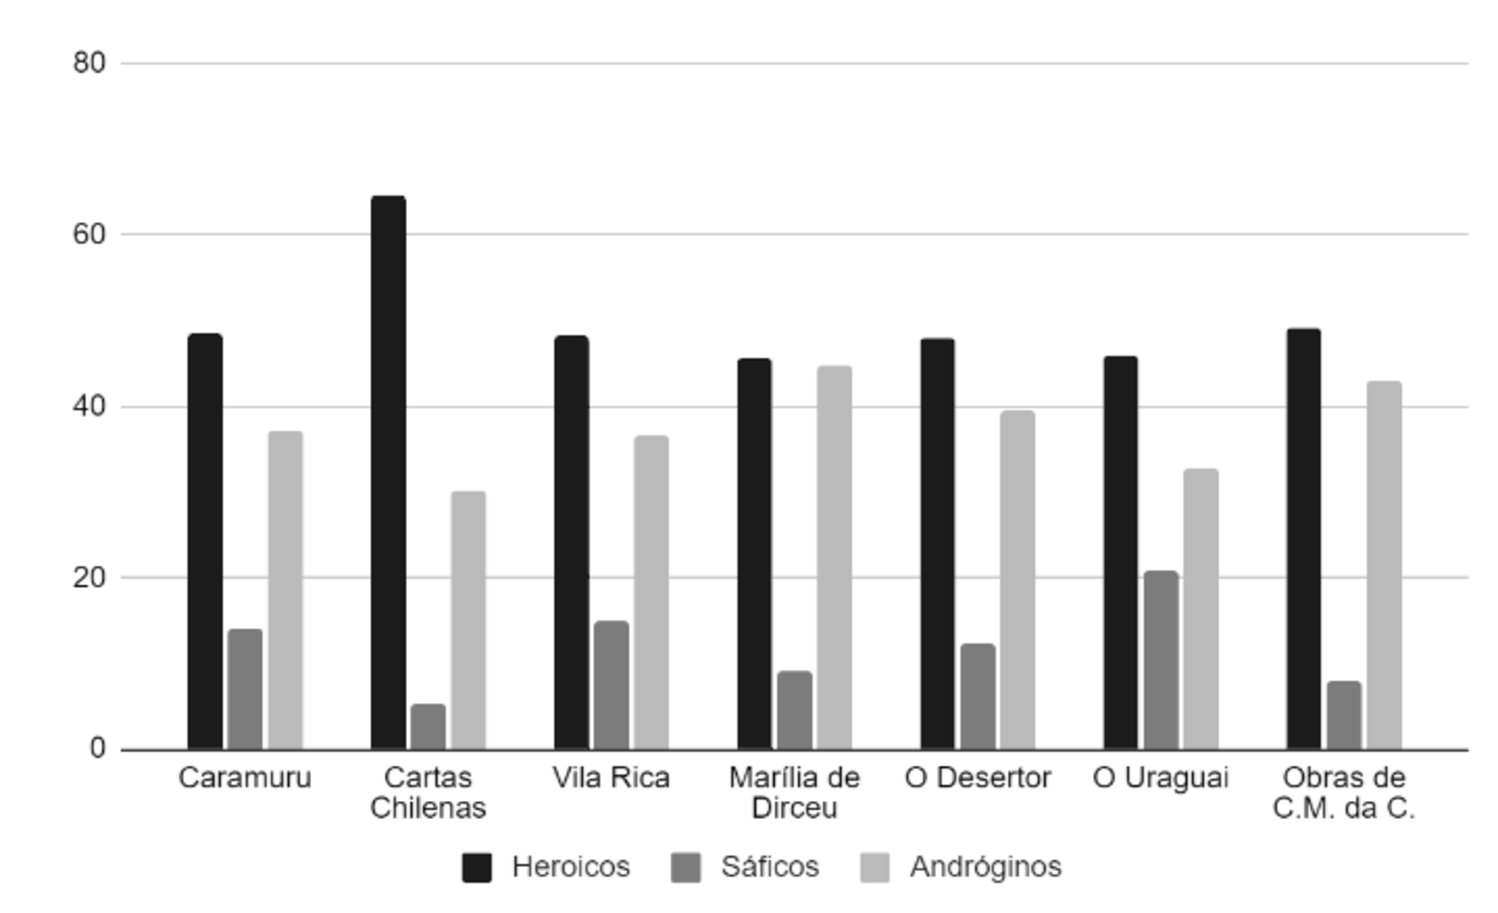
\includegraphics[width=\linewidth]{fig-002.pdf}
    \caption{Contagem individual dos tipos de decassílabo utilizados pelos neoclássicos.}
    \label{fig2}
    \source{Aoidos}
    \end{minipage}
\end{figure}

Atípico se colocado contra o plano de fundo arcádico, o emprego destacado dos decassílabos sáficos no \textit{Uraguai} não chega a chamar a atenção quando comparado ao uso que dele fizeram os nossos poetas românticos. Veja-se a \Cref{tbl2}, que descreve o percentual dos tipos de decassílabo utilizados em cada obra romântica incluída em nosso \textit{corpus}.

\begin{table}[!htbp]
\centering
\begin{threeparttable}
\caption{Disposição dos decassílabos heroicos, sáficos e andróginos nos românticos.}
\label{tbl2}
\begin{tabular}{llll}
\toprule
Obras & \multicolumn{3}{l}{Decassílabos nos românticos} \\
& Heroicos & Sáficos & Andróginos \\
\midrule
\textit{Suspiros Poéticos} &
55,6\% &
11,3\% &
32,9\% \\
Nênia &
46,8\% &
10,4\% &
39,5\% \\
\textit{Primeiros cantos} &
48,2\% &
15,2\% &
35,7\% \\
\textit{Lira dos vinte anos} &
57,6\% &
15,4\% &
26,8\% \\
\textit{Últimos cantos} &
43\% &
20,1\% &
36,5\% \\
\textit{As primaveras} &
24,5\% &
45,9\% &
29,4\% \\
\textit{Noturnas} &
42,8\% &
38,3\% &
18,5\% \\
\textit{Lírios e rosas} &
20,4\% & 
39,1\% &
39,7\% \\
\textit{Os timbiras} &
37,6\% &
20,9\% &
40,6\% \\
\textit{Crisálidas} &
35,5\% &
22,2\% &
41,9\% \\
\textit{Corimbos} &
15,4\% &
45,1\% &
38,8\% \\
\textit{Espumas flutuantes} &
38,7\% &
30\% &
31\% \\
\textit{Versos de C. de M.} &
53\% &
7,8\% &
37,7\% \\
\textit{Peregrinas} &
34,2\% &
26,3\% &
38,9\% \\
\textit{A cach. de Paulo Afo.} &
41,9\% &
28,1\% &
29,8\% \\
\textit{Os Escravos} &
39,6\% &
26,2\% &
34,2\% \\
\textit{Rosas loucas} &
35,9\% &
36,2\% &
27,7\% \\
\textit{Poesias de J. A. de C.} &
49,8\% &
20,9\% &
28,9\% \\
\textit{Fábio} &
42,2\% &
19,9\% &
37,5\% \\
\textit{Sertanejas} &
57,7\% &
9,4\% &
31,8\% \\
\textit{Quadros} &
47,8\% &
21,4\% &
30,4\% \\
\textit{Gritos da carne} &
69,2\% &
9\% &
21,5\% \\
\textit{Peregrinas} &
41\% &
31,7\% & 
26,5\% \\
\textit{Anchieta} &
57,8\% & 
12,4\% &
29,8\% \\
\textit{Estrelas errantes} &
34,8\% &
31\% &
34,2\% \\
\textit{Miosótis} &
33\% &
26,1\% &
40,7\% \\
\textit{Dias e noites} &
29,1\% &
45,7\% &
24,4\% \\
\bottomrule
\end{tabular}
\source{Aoidos.}
\end{threeparttable}
\end{table}

Em relação a essas 27 obras românticas, o uso do sáfico no \textit{Uraguai} fica dentro da média, com um valor equiparável, por exemplo, ao que se observa nos Últimos cantos e nos \textit{Timbiras} de Gonçalves Dias (20,1\% e 20,9\%, respectivamente), e supera os números de obras representativas do movimento como os \textit{Suspiros poéticos e saudades} (11,3\%), os \textit{Primeiros cantos} (15,2\%), a \textit{Lira dos vinte anos} (17,3\%) e \textit{Anchieta} (12,4\%), que possuem valores próximos aos observados nos poemas \textit{Caramuru} (14,3\%), \textit{Vila Rica} (14,8\%) e \textit{O Desertor} (12,2\%). Por outro lado, os 20,9\% do \textit{Uraguai} são largamente superados pelos altíssimos 45,9\% das Primaveras, pelos 45,7\% dos \textit{Dias e noites}, pelos 45,1\% dos \textit{Corimbos}, pelos 39,1\% de \textit{Lírios e rosas}, pelos 38,3\% das \textit{Noturnas} e assim por diante. Das 27 obras que compõem o \textit{corpus} romântico, 8 apresentam taxa superior a 30\% no emprego dos decassílabos sáficos, e 5 entre elas chegam mesmo a substituir a prevalência tradicional do verso heroico pela do sáfico, que utilizam insistentemente, por vezes em composições inteiras. São essas obras “saficomaníacas”, com valores muito acima da média do grupo (22,2\%), as principais responsáveis pela percepção de que há um emprego excessivo do sáfico entre os românticos brasileiros e pela elevação da cota dos decassílabos sáficos na soma total dos resultados, conforme vemos na \Cref{fig3}.

\begin{figure}[!h]
    \centering
    \begin{minipage}{.75\textwidth}
    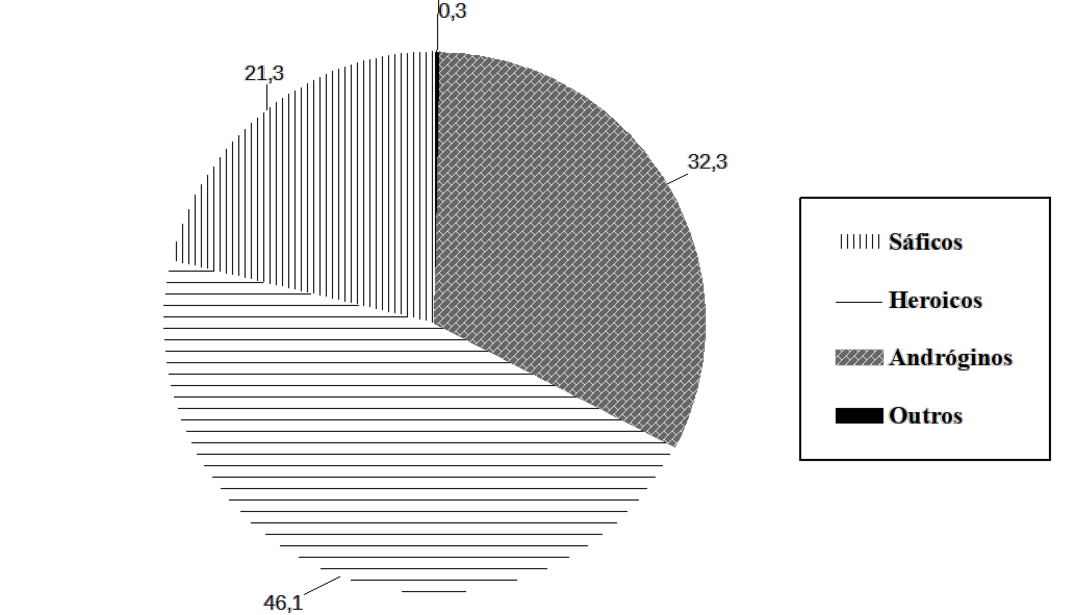
\includegraphics[width=\linewidth]{fig-003.pdf}
    \caption{Soma total dos tipos de decassílabo utilizados pelos românticos.}
    \label{fig3}
    \source{Aoidos}
    \end{minipage}
\end{figure}

Em comparação com a \Cref{fig1}, o da soma total dos tipos de decassílabos encontrados nos poetas neoclássicos, é possível perceber um crescimento de aproximadamente 75\% nos versos sáficos (de 12,2\% para 21,3\%), o que sugere uma abertura a esquemas rítmicos pouco cultivados pelos poetas do século XVIII — de fato, à exceção do \textit{Caramuru} e do \textit{Uraguai} (este notoriamente admirado, entre os românticos, pela fluidez da versificação), nenhuma obra incorporada ao grupo neoclássico chega a explorar todos os esquemas rítmicos considerados sáficos. Assim, a princípio, os resultados dessa análise de conjunto parecem corroborar a hipótese de Candido e Silva Ramos, pois o uso médio de decassílabos sáficos é, com efeito, maior entre os poetas românticos do que entre os neoclássicos. No entanto, isso não exclui a possibilidade de haver poetas românticos que se aproximem mais da média neoclássica individualmente, assim como podem existir poetas neoclássicos que se alinhem mais ao padrão romântico. A elevação da média possibilita apenas constatações de ordem tendencial. Há poetas no grupo romântico, por exemplo, em que não se observa o aumento da média sáfica, e que superam a média geral do grupo neoclássico no emprego de decassílabos heroicos: Gonçalves de Magalhães (55,6\%), Álvares de Azevedo (57,6\%), Fagundes Varela (57,8\% em \textit{Anchieta}), Celso da Cunha Magalhães (53\%), Joaquim Eleodoro (57,7\%) e José Leão (incríveis 69,2\%, ultrapassando os 64,2\% das \textit{Cartas Chilenas}). Ou seja, muito embora possamos identificar um aumento tangível no emprego médio dos versos sáficos durante o período romântico, esse aumento não configura um fenômeno geral, observável em cada caso particular, nenhuma “saficomania” amplamente compartilhada, e sim uma elevação média alavancada pelo alto índice de sáficos em algumas obras específicas.

Será que Antonio Candido tem razão ao afirmar que os poetas românticos, como um todo, incorporaram o verso sáfico “ao que havia de mais característico na sua estética” \cite[p.~36]{candido2000formacao} por razões epistemológicas, com o objetivo de combater o racionalismo excessivo do século XVIII? Não é o que indicam as nossas pesquisas, tanto mais quando comparamos os dados extraídos do corpus romântico aos que obtivemos analisando os poetas da “nova geração”, antirromânticos por definição. Veja-se na \Cref{tbl3} que descreve o percentual dos tipos de decassílabo utilizados nas obras que compõem o corpus da geração de 1870.

\begin{table}[htbp]
\centering
\begin{threeparttable}
\caption{Disposição dos decassílabos heroicos, sáficos e andróginos na geração de 1870.}
\label{tbl3}
\begin{tabular}{llll}
\toprule
Obras & \multicolumn{3}{l}{Decassílabos na geração de 1870} \\
& Heroicos & Sáficos & Andróginos \\
\midrule
\textit{Flores do Campo} &
28,5\% &
36,7\% &
34,2\% \\
\textit{Prelúdios} &
48,7\% &
31,9\% &
19\% \\
\textit{Devaneios} &
66,7\% &
13,2\% &
20,1\% \\
\textit{Canções românticas} &
47,6\% & 
12,7\% &
39,7\% \\
\textit{O caixeiro e Rosa} &
45,2\% &
15,5\% &
39,6\% \\
\textit{Hespérides} &
55\% &
10,7\% &
34,4\% \\
\textit{Auroras do sul} &
56,3\% &
18,1\% &
25,5\% \\
\textit{Cantos e lutas} &
59,1\% &
4,6\% &
36,3\% \\
\textit{Novos ideais} &
56,7\% & 
12,2\% &
31\% \\
\textit{Fanfarras} &
44,5\% &
11,8\% &
42,6\% \\
\textit{Sinfonias} &
36,7\% &
17,1\% &
45,6\% \\
\textit{Opalas} &
38,5\% &
21,7\% &
39,8\% \\
\textit{Estilhaços} &
16,3\% &
43,4\% &
39,7\% \\
\textit{Vergastas} &
37,4\% &
24,9\% &
37,5\% \\
\textit{Cantos do fim do séc.} &
47,6\% &
22\% &
29,2\% \\
\bottomrule
\end{tabular}
\source{Aoidos.}
\end{threeparttable}
\end{table}

Note-se que é bastante significativa a oscilação no emprego do decassílabo sáfico dentro da \Cref{tbl3}. Por um lado, obras como Devaneios (13,2\%), \textit{Canções românticas} (12,7\%), \textit{O Caixeiro e Rosa} (15,5\%), \textit{Hespérides} (10,7\%), \textit{Cantos e lutas} (apenas 4,6\%), \textit{Novos ideais} (12,2\%) e \textit{Fanfarras} (11,8\%) apresentam números próximos ou inferiores à média neoclássica de 12\%. Por outro, obras como \textit{Flores do campo} (36,7\%), \textit{Prelúdios} (31,9\%), \textit{Auroras do sul} (18,1\%), \textit{Sinfonias} (17,1\%), \textit{Opalas} (21,7\%), \textit{Estilhaços} (43,4\%), \textit{Cantos do fim do século} (22\%) e \textit{Vergastas} (24,9\%) tangenciam ou ultrapassam a média de 21,3\% no grupo romântico. A soma desses valores é muito semelhante, em termos proporcionais, à que obtivemos na \Cref{tbl2}, que mostra a distribuição dos decassílabos no grupo de poetas românticos, e pode ser visualizada na \Cref{fig4}.

\begin{figure}[!h]
    \centering
    \begin{minipage}{0.75\linewidth}
    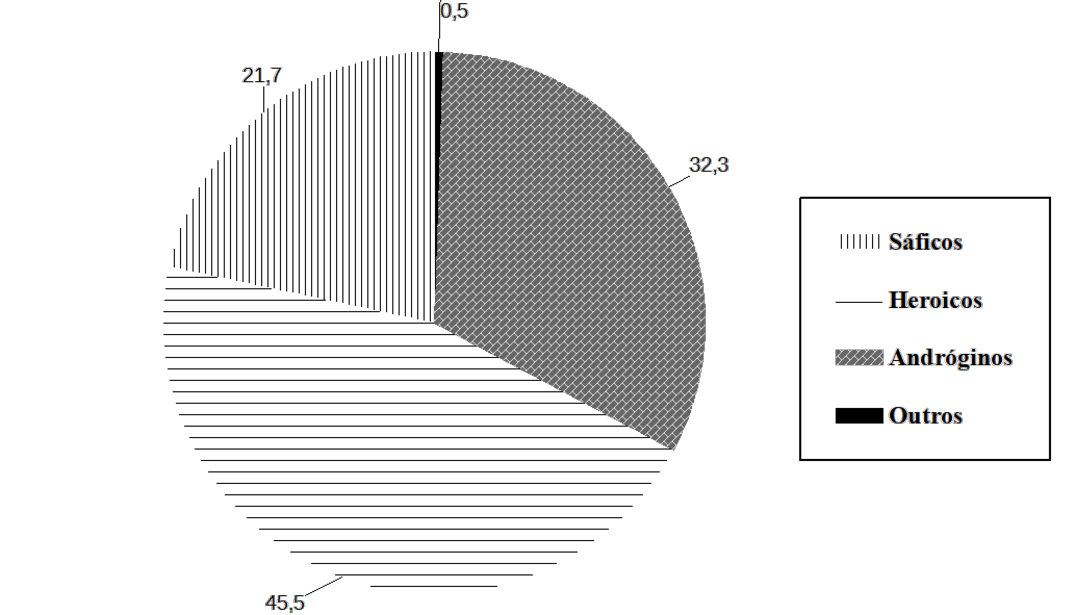
\includegraphics[width=\linewidth]{fig-004.pdf}
    \caption{Soma total dos tipos de decassílabo utilizados pela geração de 70.}
    \label{fig4}
    \source{Aoidos}
    \end{minipage}
\end{figure}

Curiosamente, a frequência do uso de versos sáficos entre os poetas românticos e os \textit{soi-disant} antirromânticos da geração de 1870 é bastante similar: 21,3\% e 21,7\%, respectivamente. As taxas de versos heroicos também são próximas, com uma redução de apenas 0,6\% na frequência de uso dos poetas de 70. Isso sugere que, embora tenha havido uma mudança significativa nos padrões rítmicos decassilábicos com a transição do paradigma neoclássico para o romântico, esses padrões permaneceram praticamente inalterados na segunda metade do século XIX, com a chegada da “geração nova”. Diante desses dados, é difícil concordar com a interpretação de Antonio Candido e José Guilherme Merquior sobre o fenômeno sáfico na poesia romântica como um contraponto ao racionalismo neoclássico. Da mesma forma, somos levados a discordar da leitura de Péricles Eugênio da Silva Ramos, que sugere uma diminuição progressiva no uso de decassílabos sáficos a partir da década de 1870, promovendo uma suposta regressão a padrões rítmicos menos centrados na 4ª sílaba. Não é isso o que se observa quando comparamos os resultados totais das gerações romântica e “antirromântica” com os dados extraídos de obras parnasianas. Vejamos os dados na \Cref{tbl4}.

\begin{table}[!htbp]
\centering
\begin{threeparttable}
\caption{Disposição dos decassílabos heroicos, sáficos e andróginos nos parnasianos.}
\label{tbl4}
\begin{tabular}{llll}
\toprule
Obras & \multicolumn{3}{l}{Decassílabos nos parnasianos} \\
& Heroicos & Sáficos & Andróginos \\
\midrule
\textit{Sonetos e poemas} &
35,7\% &
18,4\% &
45,8\% \\
\textit{Sonetos e rimas} &
19,9\% &
21,7\% &
58\% \\
\textit{Versos e versões} &
33,6\% &
18,1\% &
47,8\% \\
\textit{Versos de um simp.} &
25,3\% &
26,7\% &
47,8\% \\
\textit{Poesias de A. de Oli.} &
36,1\% &
17,9\% &
46\% \\
\textit{Mármores} &
30\% &
22,2\% &
48\% \\
\textit{Cromos} &
38\% &
20,4\% &
41,6\% \\
\textit{Meridionais} &
32,5\% &
18,8\% &
48,6\% \\
\textit{Poesias de O. Bilac} &
34,8\% &
24,9\% &
40,2\% \\
\textit{Vibrações} &
31,3\% &
26,4\% &
42,1\% \\
\textit{Ementário} &
29,1\% &
22,5\% &
47,4\% \\
\textit{Tarde} &
45,7\% &
20\% &
33,7\% \\
\textit{Esfinges} &
30,9\% &
21\% &
48,3\% \\
\textit{Poes. de R. Correia} &
36,9\% &
19,2\% &
43,4\% \\
\bottomrule
\end{tabular}
\source{Aoidos.}
\end{threeparttable}
\end{table}

Com relação ao emprego dos versos sáficos, os valores apresentados pela \Cref{tbl4} revelam uma ambiguidade interessante. Por um lado, notamos que as obras parnasianas nunca ultrapassam a casa das vintenas (\textit{Versos de um simples}, de Guimarães Passos, tem a maior proporção, com 26,7\%), ficando muito aquém dos 45,9\% e 43,4\% observados, respectivamente, nos grupos romântico e da geração de 1870. Por outro lado, nenhuma obra parnasiana apresenta uma proporção de versos sáficos inferior à encontrada nas \textit{Poesias} de Alberto de Oliveira (17,9\%), um valor consideravelmente superior ao de várias obras do romantismo e da geração de 1870, como \textit{Versos}, de Celso de Magalhães (7,8\%), \textit{Suspiros poéticos} (11,3\%), \textit{Sertanejas} (9,4\%), \textit{Gritos da Carne} (9\%), \textit{Anchieta} (12,4\%), \textit{Canções românticas} (12,7\%), \textit{Hespérides} (10,7\%),\textit{ Cantos e Lutas} (4,6\%), \textit{Novos ideais} (12,2\%) e \textit{Fanfarras} (11,8\%). Isso indica que, ao contrário de outros grupos, todas as obras parnasianas mantêm-se próximas da média geral. A diferença entre a menor e a maior proporção de versos sáficos no grupo parnasiano é de apenas 9 pontos, enquanto as variações nos grupos neoclássico, romântico e da geração de 1870 são, respectivamente, de 15, 38 e 39 pontos. Não há poetas parnasianos particularmente inclinados ao verso sáfico, mas também não há poetas que o rejeitem. Esse equilíbrio curioso faz com que, na soma total dos dados da \Cref{tbl4}, a incidência média de decassílabos sáficos permaneça praticamente igual à observada nos grupos romântico e da nova geração (\Cref{fig5}).

\begin{figure}[!h]
    \centering
    \begin{minipage}{0.75\linewidth}
    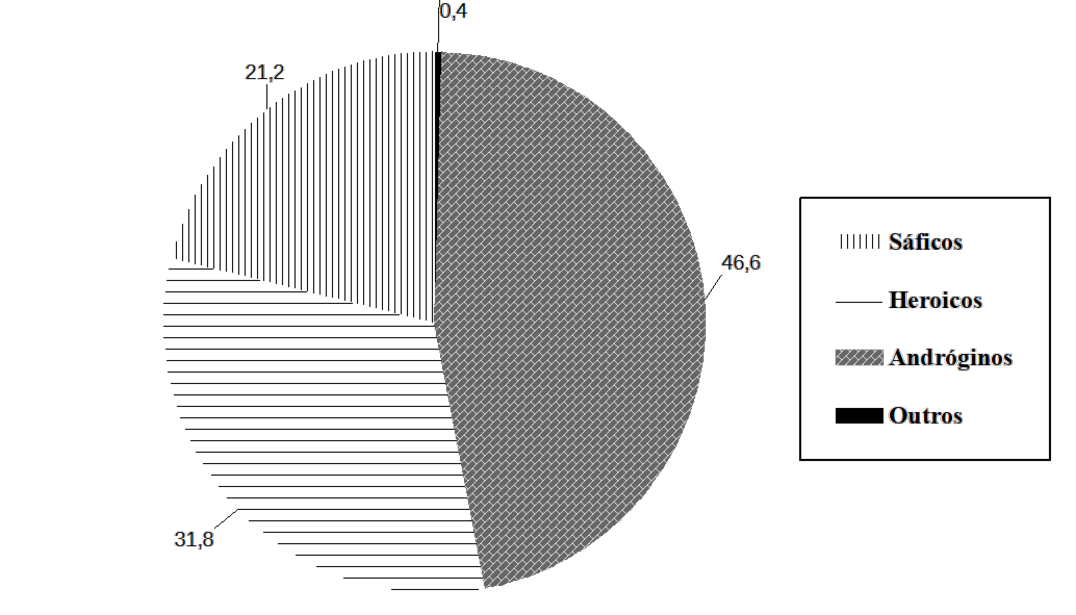
\includegraphics[width=\linewidth]{fig-005.pdf}
    \caption{Soma total dos tipos de decassílabo utilizados pelos parnasianos.}
    \label{fig5}
    \source{Aoidos}
    \end{minipage}
\end{figure}

Na \Cref{fig5}, o que chama a atenção não é a ocorrência dos versos sáficos, mas a redução drástica dos heroicos em favor dos andróginos, indicando uma preferência marcante na poética parnasiana pela acentuação simultânea nas 4ª e 6ª sílabas. Note-se que, excetuando-se o livro \textit{Tarde}, de Olavo Bilac, todos os livros dos poetas parnasianos ultrapassam a marca dos 40\% de versos andróginos, isto é, de decassílabos cuja decisão entre heroico e sáfico depende não apenas dos versos anteriores e posteriores, mas também da subjetividade do leitor. Fica a questão: seria esta ambiguidade de ritmo empregada conscientemente, a fim de gerar uma maior riqueza rítmica? A pergunta é válida, pois, ao comparar os estilos simbolista e parnasiano, \textcite[p.~28]{ramos1965poesia} afirma que “o ritmo do primeiro é fluido e musical, até irregular, de vez em quando, o do segundo é rígido, regular e às vezes confragoso”. Seriam os parnasianos mais harmônicos e suaves do que supunha o crítico?

Vejamos agora, a fim de concluir de maneira sintética a discussão dos dados obtidos em nossa pesquisa, uma sobreposição linear e cronológica das \Cref{fig1,fig2,fig3,fig4,fig5}, quer dizer, uma sobreposição dos gráficos de soma total dos tipos de decassílabos utilizados por cada grupo analisado.

\begin{figure}[!h]
    \centering
    \begin{minipage}{0.85\linewidth}
    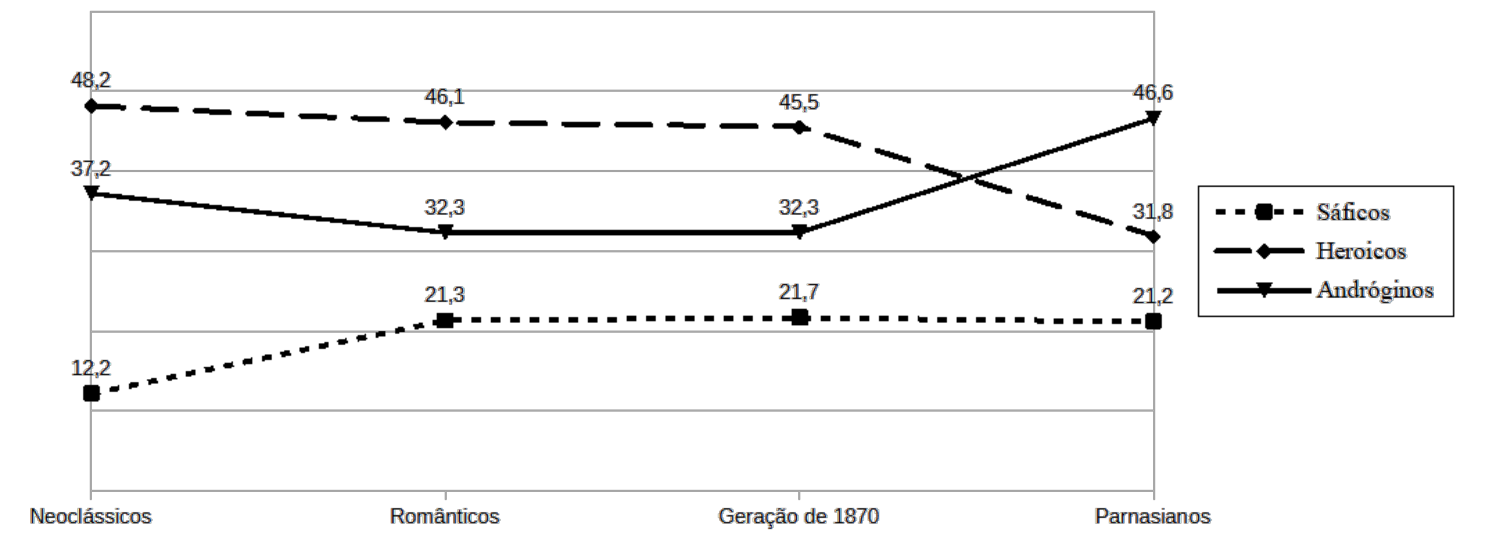
\includegraphics[width=\linewidth]{fig-006.pdf}
    \caption{Progressão do uso de decassílabos dos neoclássicos aos parnasianos.}
    \label{fig6}
    \source{Aoidos}
    \end{minipage}
\end{figure}

A \Cref{fig6} revela ao menos três movimentos importantes na evolução métrica da poesia brasileira ao longo do século XIX. Em primeiro lugar, ele aponta um progressivo declínio no uso de versos heroicos, com uma queda de aproximadamente 30\% (de 45,5\% para 31,8\%) entre a geração de 1870 e a escola parnasiana, evidenciando uma mudança comportamental no repertório rítmico dos poetas dessa época, o que confere maior maleabilidade aos seus versos. Em sentido contrário, os versos andróginos apresentam um crescimento expressivo de 44\% (de 32,3\% para 46,6\%) no mesmo intervalo, sugerindo uma clara preferência dos parnasianos pelo padrão ambíguo em detrimento dos ritmos estritamente heroicos. Já o dado mais relevante para a nossa análise é o aumento de 75\% (de 12,2\% para 21,3\%) no uso dos versos sáficos na transição do século XVIII para o XIX, o que, em parte, corrobora as interpretações de Candido, Silva Ramos e Merchior. No entanto, essa correlação se enfraquece na passagem do grupo romântico para os grupos pós-românticos (geração de 70 e parnasianismo), pois a proporção no uso do verso sáfico se estabiliza com a entrada no Oitocentos, o que impede a sua caracterização como um traço distintivo da poética romântica, exceto se considerarmos apenas os dois primeiros grupos analisados.

\section{Conclusão}\label{sec-fmt-manuscrito}
Foi nosso objetivo, neste artigo, reavaliar a conhecida hipótese segundo a qual o verso sáfico poderia ser considerado um traço distintivo da poética romântica brasileira. A partir de uma análise quantitativa conduzida por meio da ferramenta de processamento automático de textos Aoidos, verificou-se que, embora se observe um aumento na utilização do verso sáfico na transição do século XVIII para o XIX, tal incremento não se restringe ao romantismo. O verso sáfico mantém-se presente de modo constante ao longo de todo o século XIX, abrangendo também a geração de 1870 e o parnasianismo. Assim, nossa pesquisa aponta que a atribuição do sáfico como marca distintiva da poética romântica não se sustenta, visto que não há uma variação significativa que justifique a sua associação exclusiva a esse movimento literário.



\printbibliography\label{sec-bib}
%conceptualization,datacuration,formalanalysis,funding,investigation,methodology,projadm,resources,software,supervision,validation,visualization,writing,review
\begin{contributors}[sec-contributors]
\authorcontribution{Gabriel Esteves}[conceptualization,datacuration,formalanalysis,investigation,writing,review]
\authorcontribution{Leandro Scarabelot}[conceptualization,datacuration,formalanalysis,investigation,writing,review]
\authorcontribution{Ana Paula Nunes de Sousa}[conceptualization,datacuration,formalanalysis,investigation,writing,review]
\end{contributors}
\end{document}


